\documentclass[aspectratio=169]{beamer}


\usepackage[utf8]{inputenx} % For æ, ø, å
\usepackage{csquotes}       % Quotation marks
\usepackage{microtype}      % Improved typography
\usepackage{amssymb}        % Mathematical symbols
\usepackage{mathtools}      % Mathematical symbols
\usepackage[absolute, overlay]{textpos} % Arbitrary placement
\setlength{\TPHorizModule}{\paperwidth} % Textpos units
\setlength{\TPVertModule}{\paperheight} % Textpos units
\usepackage{tikz}
\usetikzlibrary{overlay-beamer-styles}  % Overlay effects for TikZ

\usepackage{hyperref}
\usepackage{svg}

\usepackage{color, soul, xcolor} % Colored text and highlighting, respectively
\usepackage{tikz-cd} % For commutative diagrams
\usepackage{tikz-3dplot}
\usetikzlibrary{angles}
\RequirePackage{pgfplots}
\usepackage{mathtools}
\usepackage{answers}
\usepackage{setspace}
\usepackage{graphicx}
\usepackage{enumerate}
\usepackage{multicol}
\usepackage{mathrsfs}
\usepackage{amsmath,amsthm,amssymb}
\usepackage{marvosym,wasysym} %fucking smileys
\usepackage{float}
\usepackage{morefloats}
\usepackage{pgf,tikz}
\pgfplotsset{compat=1.15}
\usepackage{mathrsfs}
\usetikzlibrary{arrows}
\usepackage{subcaption}
\usepackage[most]{tcolorbox}
\tcbuselibrary{theorems}
\usepackage{fancyvrb}
\usepackage{longtable,booktabs}
\usepackage{stackrel}

\newcommand{\vecx}{\boldsymbol{\vec{x}}}
\newcommand{\vecf}{\boldsymbol{\vec{f}}}
\newcommand{\xdot}{\boldsymbol{\dot{\vec{x}}}}



\usetheme{UiB}

\definecolor{lighter_csu_green}{RGB}{60,133,77}
\newcommand\boldgreen[1]{\textcolor{lighter_csu_green}{\emph{\textbf{#1}}}}


\author{Colin Roberts}
\setbeamercolor{title}{fg=white} 
\title{A Multiscale approach to modeling the municipal spread of COVID-19}
\setbeamercolor{subtitle}{fg=white} 
\subtitle{}


\begin{document}

\begin{frame}{}
\vfill
    Joint work with
    \begin{itemize}
        \item Elijah Pivo, MIT Institute for Data, Systems, and Society.
        \item Claire Valva, NYU Courant Center for Atmosphere and Ocean Science.
    \end{itemize}
    \vfill
\end{frame}

\begin{frame}{}
\vfill
\center
    Note that the phrase,\\
    \vspace*{.5cm}
    \boldgreen{``All models are wrong, but some are useful"}\\
    \vspace*{.5cm}
    is in play.
\vfill 
\end{frame}

\begin{frame}{Outline}
\vfill
\center
    \begin{enumerate}[1.]
    \pause
        \item Discuss agent based modeling.
        
        \pause
        \item Revisit ODEs and review the SIR model.
        
        \pause
        \item Interlude on parameter estimation using data assimilation.
        
        \pause
        \item Describe the multiscale modeling approach.
        
        \pause
        \item Results
        \begin{enumerate}[a.]
        \pause
            \item (Agent): contact rate in the university.
            \begin{enumerate}[i.]
            \pause
                \item Class sizes.
                
                \pause
                \item Class periods.
            \end{enumerate}
            \pause
            \item (Compartmental): municipal disease spread.
            \begin{enumerate}[i.]
            \pause
                \item University-city coupling.
            \end{enumerate}
            \pause
            \item (Multiscale): interactions involving both levels.
            \begin{enumerate}[i]
            \pause
                \item Staggered schedules.
                
                \pause
                \item Quarantining/presymptomatic.
            \end{enumerate}
        \end{enumerate}
    \end{enumerate}
\vfill
\end{frame}

\section{Preliminaries}

\begin{frame}{Question}
\vfill
    \center
    \pause
    How do schools and universities impact the spread of COVID-19 in the surrounding community?
\vfill
\end{frame}


\begin{frame}{Ideas}
    \vfill
    \center
    \pause
    \begin{itemize}
        \item Use an (non deterministic and heterogeneous) agent based approach.
        \pause
        \item Use a (deterministic and homogeneous) compartmental model approach.
    \end{itemize} 
   \vfill
\end{frame}

\subsection{Agent based modeling}

\begin{frame}{Agent based simulations}
    \vfill
    \begin{itemize}
    \pause
        \item Treat every individual as a single \boldgreen{agent} (entity).
        \pause
        \item Describe every agent's schedule, movement, and infection status at every instant in time.
        \pause
        \item Let agents interact with one another and keep track of the disease progression.
    \end{itemize}
    \vfill
\end{frame}

\begin{frame}{Examples}
    \vfill
    \begin{itemize}
    \pause
        \item Particle based simulations. (3Blue1Brown)
        \vspace*{1cm}
        \begin{figure}[H]
            \centering
            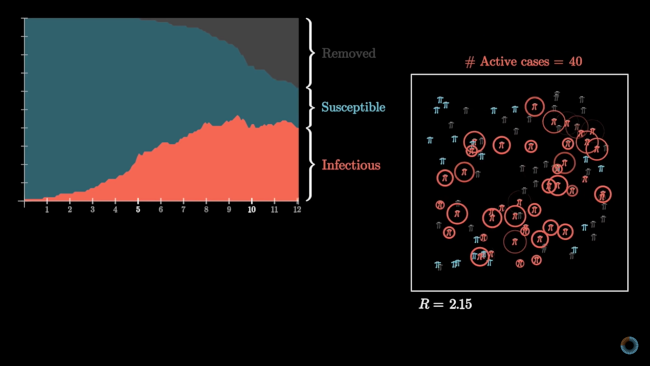
\includegraphics[width=.5\textwidth]{figures/3b1b_covid_agent.png}
        \end{figure}
    \end{itemize}
    \vfill
\end{frame}

\begin{frame}{Examples}
    \vfill
    \begin{itemize}
    \pause
        \item Network based simulations. (covasim)
        \vspace*{.75cm}
                \begin{figure}[H]
                    \centering
                    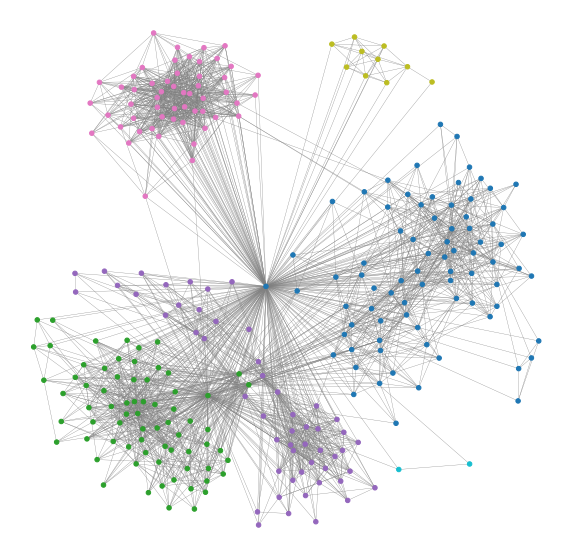
\includegraphics[width=.4\textwidth]{figures/network_diagram.png}
                \end{figure}
            \end{itemize}
            \vfill
\end{frame}

\begin{frame}{Benefits}
    \vfill
    \textbf{\underline{Benefits of agent models:}}
    \begin{itemize}
        \pause
        \item Heterogeneous social structure.
        \pause
        \item Stochastic.
        \pause
        \item (Typically) less ad-hoc parameter tuning.
    \end{itemize}
    \vfill
\end{frame}

\begin{frame}{Drawbacks}
    \vfill
    \textbf{\underline{Drawbacks of agent models:}}
    \begin{itemize}
        \pause
        \item Complicated to design.
        \pause
        \item Slow to run.
        \pause
        \item Stochastic nature requires ensembles to generate statistics.
    \end{itemize}
    \vfill
\end{frame}

\subsection{Compartmental modeling}

\begin{frame}{Compartmental (ODE) based simulations}
    \vfill
    \begin{itemize}
    \pause
        \item Consider an entire homogeneous population.
        \pause
        \item Ignore individualistic behavior for course-grained homogeneity.
        \pause
        \item Assume efficient and homogeneous mixing.
    \end{itemize}
    \vfill
\end{frame}

\begin{frame}{Example}
    \vfill
    \begin{itemize}
    \pause
        \item SIR Model (Kermack and McKendrick, 1927)
        \vspace*{1cm}
        \begin{figure}[H]
            \centering
            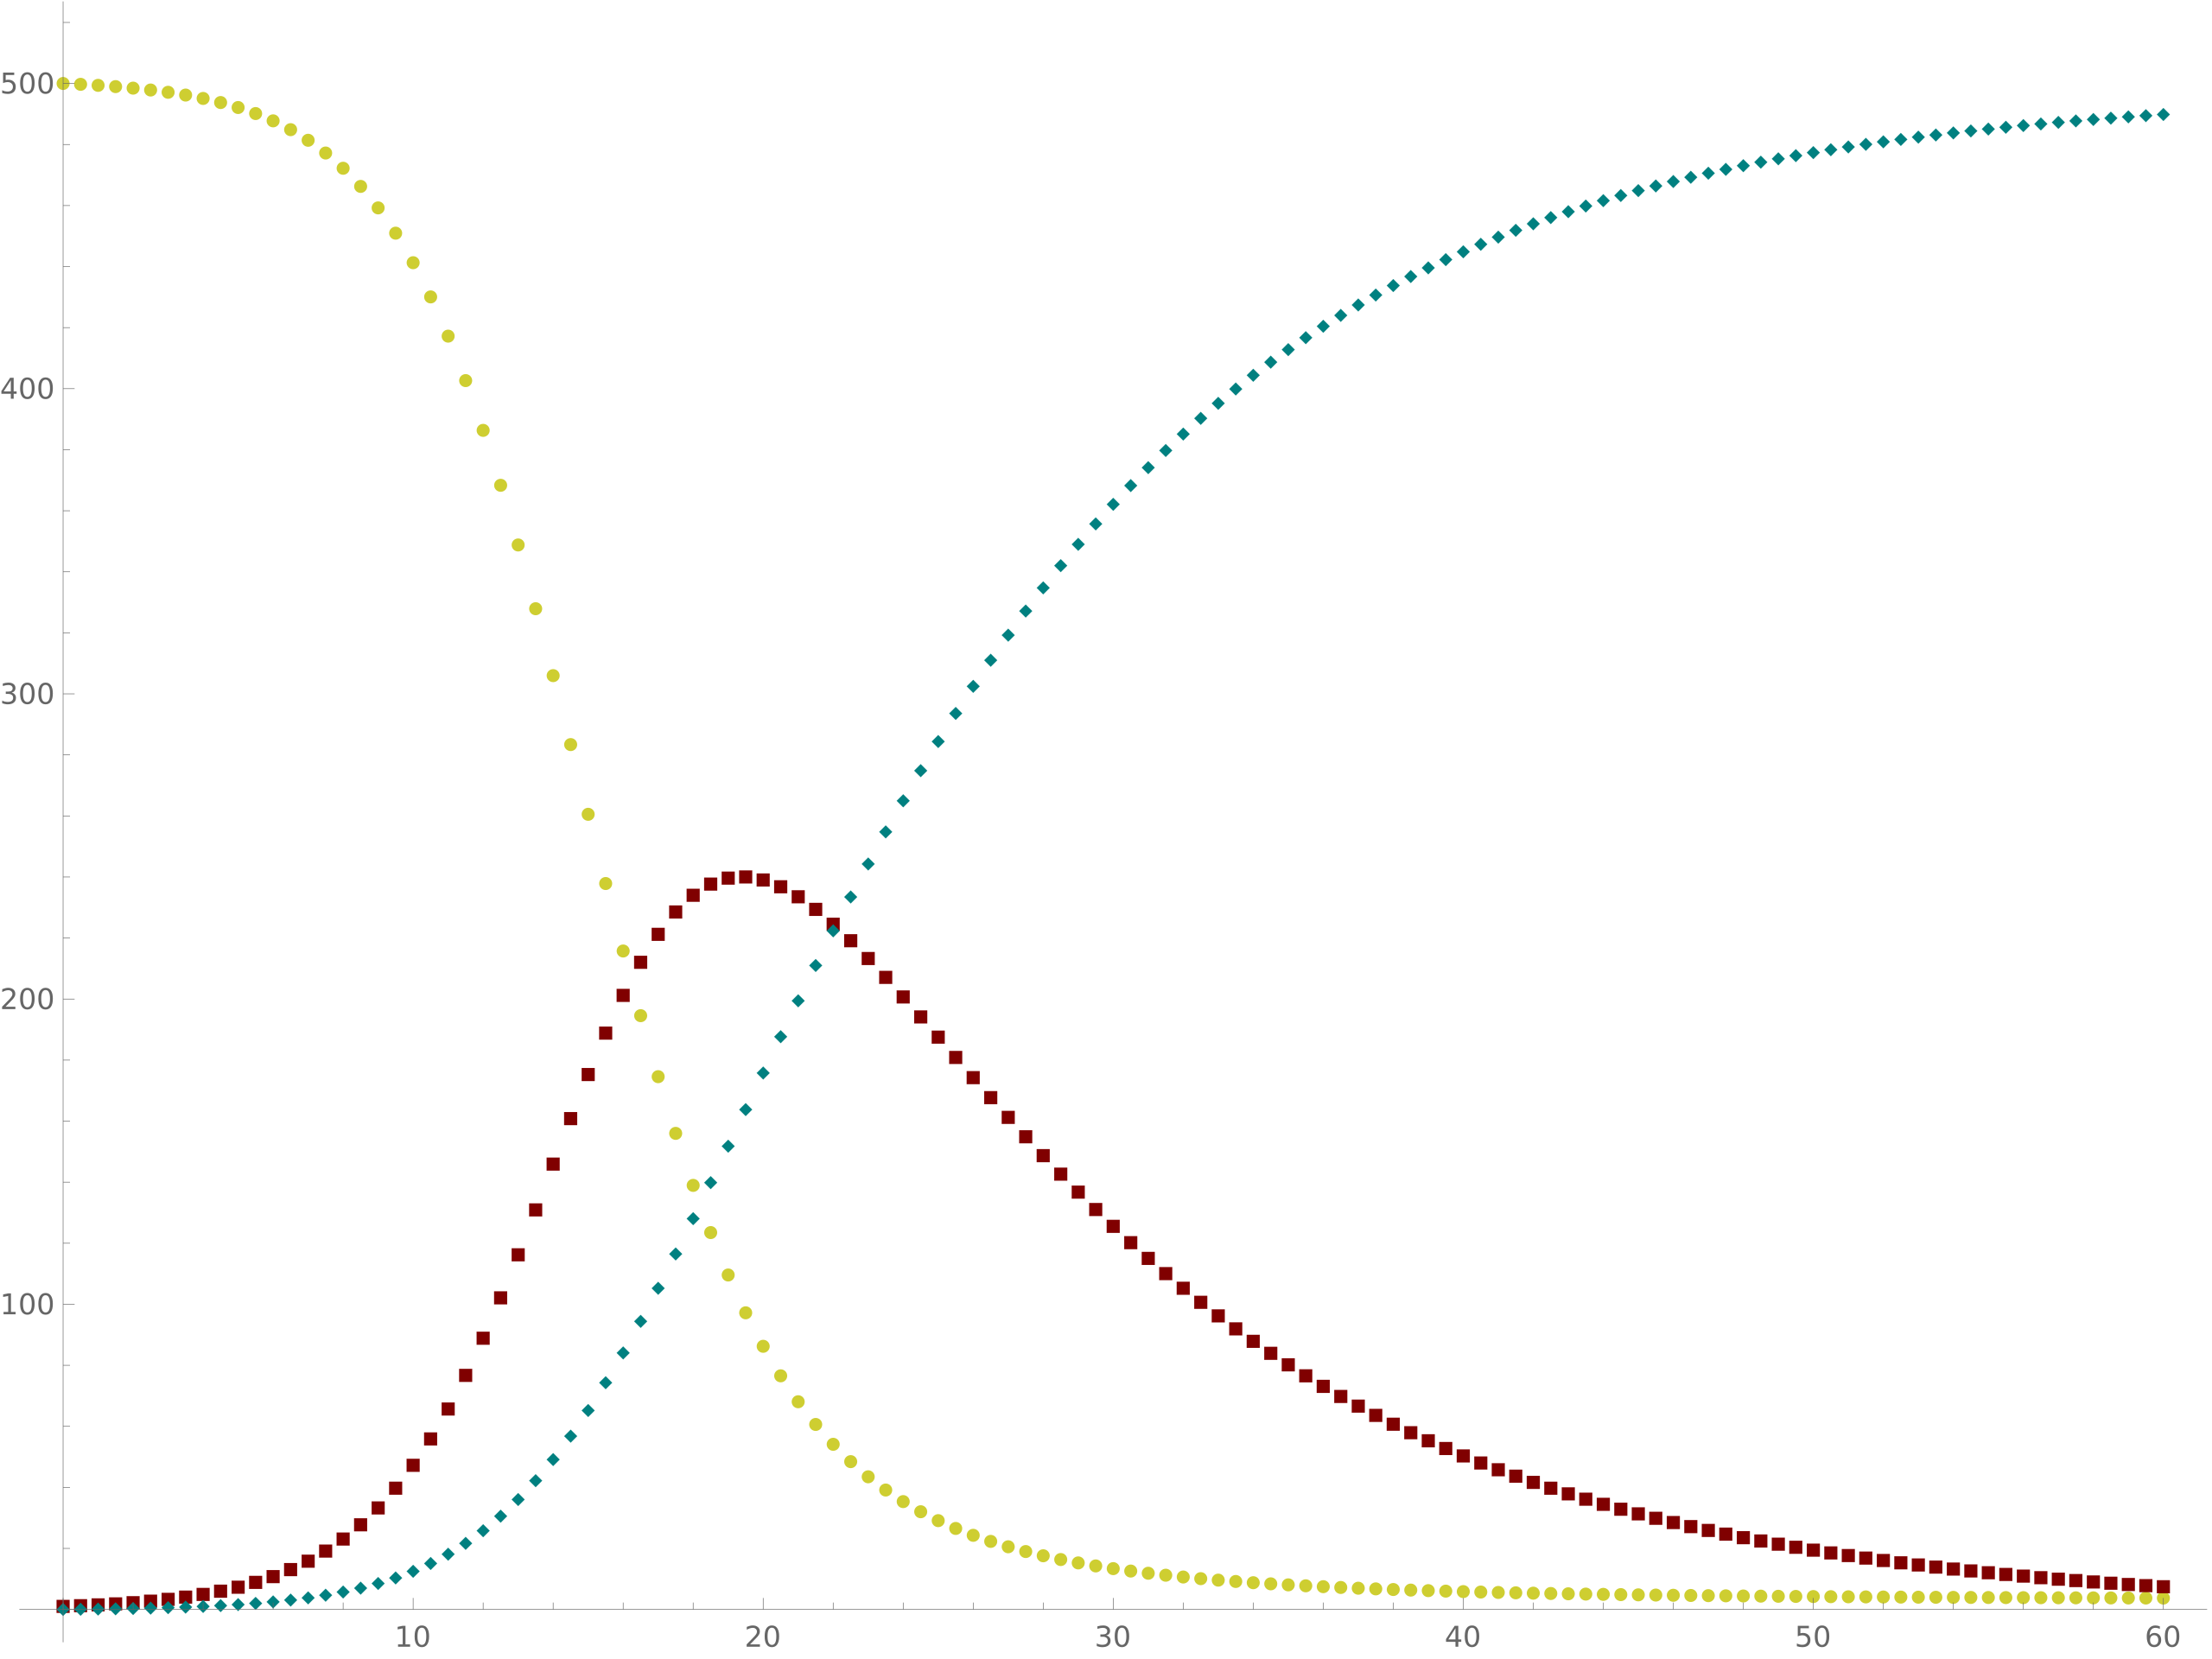
\includegraphics[width=.5\textwidth]{figures/sir_curves.png}
        \end{figure}
    \end{itemize}
    \vfill
\end{frame}

\begin{frame}{SIR equations}
    \vfill
    \pause
    We can write \emph{any} ODE as a first order update of a state $\vecx$ by
    \[
    \xdot = \vecf(t,\vecx).
    \]
    The SIR equations then read
    \[
    \begin{pmatrix} \dot{S} \\ \dot{I} \\ \dot{R} \end{pmatrix} = \begin{pmatrix} -\beta C \frac{I}{N} \\ +\beta C \frac{I}{N} - \gamma I \\ + \gamma I \end{pmatrix}, 
    \]
    where $S$, $I$, and $R$ denotes the \boldgreen{susceptible}, \boldgreen{infected}, and \boldgreen{removed} populations respectively. Note, $N=S+I+R$ is the total (conserved) population size.
    \vfill
\end{frame}

\begin{frame}{Relation to chemistry}
\vfill
    The equation
    \[
    \dot{S} = -\beta C \frac{I}{N},
    \]
    can be thought of as a first order chemical reaction
    \[
    S + I \to ...
    \]
    \pause
    \begin{itemize}  
        \item $C$ describes how many contacts with other molecules per unit time species $S$ experiences.
        \pause
        \item $\frac{I}{N}$ is the proportion of these molecules of the proper type.
        \pause
        \item $\beta$ is the likelihood of reaction.
    \end{itemize}
\vfill    
\end{frame}

\begin{frame}{Understanding SIR parameters}
    \vfill
    \pause
    The parameters $\beta$, $C$, and $\gamma$ can be thought of as:
    \begin{itemize}
    \pause
        \item $\beta \in [0,1]$ is likelihood of transmission.
        \pause
        \item $C \in [0,\infty)$ is the contact rate.
        \pause
        \item $\gamma \in [0,\infty)$ is the recovery + death rate.
    \end{itemize}
    \vfill
\end{frame}

\begin{frame}{Benefits}
    \vfill
    \textbf{\underline{Benefits of compartmental models:}}
    \begin{itemize}
        \pause
        \item Easy to analyze and compute.
        \pause
        \item Captures large scale behavior.
    \end{itemize}
    \vfill
\end{frame}

\begin{frame}{Drawbacks}
    \vfill
    \textbf{\underline{Drawbacks of compartmental models:}}
    \begin{itemize}
        \pause
        \item Homogeneous.
        \pause
        \item Deterministic.
        \pause
        \item Ad-hoc parameter changes.
    \end{itemize}
    \vfill
\end{frame}

\subsection{Multiscale modeling}

\begin{frame}{Multiscale modeling}
    \vfill
    \begin{itemize}
    \pause
        \item Interesting dynamics for a single system can take place on various spatio-temporal scales.
        \pause
        \item Small scale interactions drive large scale phenomenon.
        \pause
        \item Couple together small and large scale models to study complicated systems.
        \pause
        \item E.g., quantum mechanics $\to$ molecular dynamics $\to$ kinetic theory $\to$ statistical mechanics $\to$ thermodynamics.
    \end{itemize}
    \vfill
\end{frame}

\begin{frame}{Idea}
    \vfill
    Can we couple an agent based model alongside a compartmental model to remove the drawbacks and gain benefits?
    \vfill
\end{frame}

\section{Multiscale COVID-19 modeling}

\begin{frame}{Hierarchical compartmental model}
\vfill
\pause
Assume the following:
    \begin{itemize}
    \pause
        \item Two coupled SIR systems $S_1$, $I_1$, $R_1$, and $S_2$, $I_2$, and $R_2$.
        \pause
        \item System 1 refers to the university students and System 2 all other citizens in the city that aren't university members.
        \pause
    \end{itemize}
        \begin{figure}[H]
            \centering
            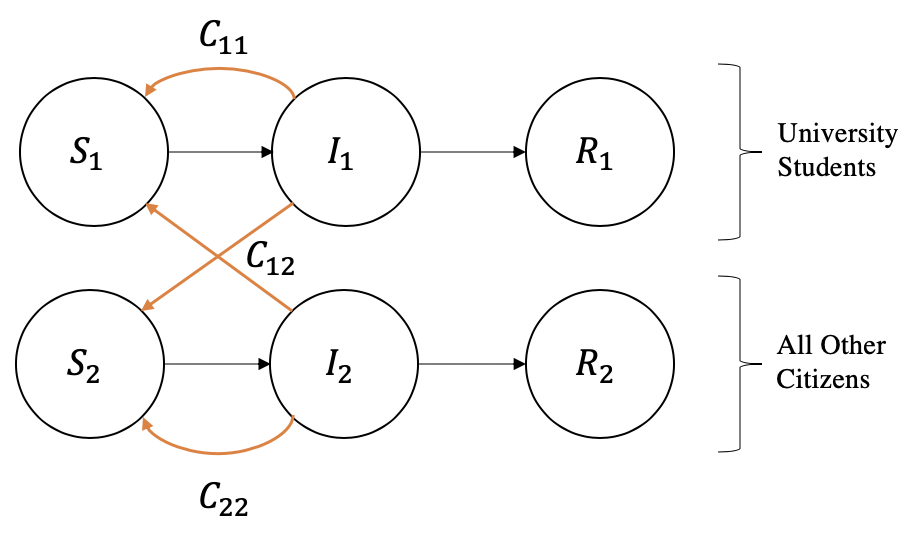
\includegraphics[width=.6\textwidth]{figures/compartmental_sir.png}
        \end{figure}
        \vfill
\end{frame}

%\begin{frame}{Hierarchical compartmental model}
%\vfill
%\pause
%    In general, for $n$ systems, we have the equations
%    \[
%    \begin{pmatrix} \dot{S}_i \\ \dot{I}_i \\ \dot{R}_i \end{pmatrix} = \begin{pmatrix} -\beta S_i \sum_j C_{ij} \frac{I_j}{N_j} \\ +\beta  S_i \sum_j C_{ij} \frac{I_j}{N_j} - \gamma I_j \\ + \gamma I_j \end{pmatrix}.
%    \]
%    \pause
%    In this case, the contact rate $C$ becomes the \boldgreen{contact matrix} $C_{ij}$ that describes the contact rate between the systems $i$ and $j$. Note $C_{ij}$ is symmetric.
%    \vfill
%\end{frame}
%
%\begin{frame}{Aggregating systems}
%    \vfill
%    \begin{itemize}
%    \pause
%    \item Many systems may comprise a larger system (e.g., System 1 + System 2 from before comprise the entire city).
%    \pause
%    \item This decomposition allows us to aggregate larger system dynamics by summing over relevant systems.
%    \begin{itemize}
%    \vfill
%\end{frame}
%
%\begin{frame}{Adding complexity}
%\vfill
%SIR is lacking.  We prefer the SEQIRD compartmental model governed by
%\[
%\begin{pmatrix} \dot{S}_i \\ \dot{E}_i \\ \dot{Q}_i \\ \dot{I}_i \\ \dot{R}_i \\ \dot{D}_i \end{pmatrix} = \begin{pmatrix} -\beta S_i \sum_j C_{ij} \frac{I_j}{N_j} \\ \beta S_i \sum_j C_{ij} \frac{I_j}{N_j} - (\gamma_I - \gamma_Q)E_i \\ \gamma_I E_i - (\lambda + \kappa)I_i \\ \gamma_Q E_i - (\lambda + kappa) Q_i \\ \lambda(I_i + Q_i) \\ \kappa (I_i + Q_i) \end{pmatrix}
%\]
%
%\end{frame}



\begin{frame}{Acknowledgements}
\vfill
\begin{figure}
     \centering
     \begin{subfigure}[b]{0.45\textwidth}
         \centering
         
\includegraphics[width=\textwidth]{figures/mcrn_logo.png}
     \end{subfigure}
     \hfill
     \begin{subfigure}[b]{0.3\textwidth}
         \centering
         
\includegraphics[width=\textwidth]{figures/nsf_logo.png}
     \end{subfigure}
     \\
     \vspace*{1cm}
     \begin{subfigure}[b]{0.8\textwidth}
         \centering
         
\includegraphics[width=\textwidth]{figures/aim_logo.jpg}
     \end{subfigure}
\end{figure}
\vfill
\end{frame}




\end{document}